\documentclass[letterpaper,11pt]{report}
% Change margins to 1 inch on all sides
\addtolength{\oddsidemargin}{-.875in}
\addtolength{\evensidemargin}{-.875in}
\addtolength{\textwidth}{1.75in}
\addtolength{\topmargin}{-.875in}
\addtolength{\textheight}{1.75in}
\usepackage{float}
\usepackage{graphicx}
\usepackage{footnote}
\usepackage{longtable}
\usepackage{multirow}
\usepackage{tablefootnote}
\usepackage{tabularx}
\usepackage{url}
\DeclareGraphicsExtensions{.pdf,.png,.jpg}

%%%%%%%%%%Start of report
\begin{document} 
\begin{savenotes}
\pagestyle{plain}
\title{CS896 Introduction to Web Science\\Fall 2013\\Report for Assignment 7}
\author{Corren G. McCoy}
 
\date{November 7, 2013}
\maketitle

\renewcommand*\thesection{\arabic{section}}
\setcounter{section}{0}

\setcounter{tocdepth}{4}
\tableofcontents
 \listoffigures
\newpage


%%%%%%%%%%Chapter Exercises
\section{Question 1}
\subsection{Problem}Using D3, create a graph of the karate club before and after the split. Weight the edges with the data from:  \url{http://vlado.fmf.uni-lj.si/pub/networks/data/ucinet/zachary.dat}. Have the transition from before/after the split occur on a mouse click.

\subsection{Response}The input data for Zachary's karate club was obtained from the Nexus Network Repository (\url{http://www.nexus.igraph.org/api/dataset_info?id=1&format=html}) in GraphML format. In addition to the nodes and links, their file also contains attributes for edge weight and associated faction (i.e., club president (John A.), karate instructor (Mr. Hi)) of the club member after the split. A snippet of the XML from the graph file is shown below:

\begin{verbatim}
    [nodes] => Array
        (
            [0] => stdClass Object
                (
                    [Faction] => 1
                    [id] => n12
                    [name] => Actor 13
                )
\end{verbatim} 
\begin{verbatim}
    [links] => Array
        (
            [0] => stdClass Object
                (
                    [source] => 0
                    [target] => 26
                    [weight] => 1
                )
\end{verbatim}

\indent{}Since GraphML is not a file format that is natively handled by D3, we used Python to convert the GraphML to a CSV file. The Python source, shown in Appendix \ref{chap:Python}, performs the following tasks:
\begin{itemize}
\item Read the GraphML file;
\item Convert the file to JSON using the utilities in the NetworkX library;
\item Read and parse the JSON file;
\item Save the nodes and links in two Python dictionary objects;
\item The \emph{source} and \emph{target} in the links array are actually index pointers into the nodes array. Therefore, we must correlate the pointers to retrieve the correct node ID and name attribute. It should be noted that despite the prefix of \emph{Actor}, the node number corresponds to Zachary's nomenclature for identifying each student in the karate club;
\item Write the name attribute of the source and target nodes and the faction to a CSV file. 
\end{itemize}

\indent{}The CSV file was used as input data for processing using the D3\footnote{\url{http://d3js.org/}} JavaScript library. The data includes the source node, target node, faction of the source and faction of the target. A snippet of the generated data file is shown below: 

\begin{verbatim}
     source,target,sfaction,tfaction
     Actor 13,Mr Hi,1,1
     Actor 13,Actor 4,1,1
     Actor 14,Mr Hi,1,1
     Actor 14,Actor 2,1,1
     Actor 14,Actor 3,1,1
     Actor 14,Actor 4,1,1
\end{verbatim}

We chose to visualize the karate club as a Force Layout diagram. This type of diagram is well-suited for networks since it allows us to easily represent the nodes and links between nodes (edges) as a graph. The D3 source, shown in Appendix \ref{chap:D3}, performs the following tasks:
\begin{itemize}
\item Read and parse the CSV file;
\item Create a \emph{nodes} and \emph{links} array using the source and target data from the CSV file;
\item Assign a color to each node based on its associated faction;
\item Establish the configuration parameters for the visualization (e.g., height, width, radius); 
\item Invoke the D3 construct which creates the force layout on our screen canvas;
\item We experimented with combinations of values for the gravity, link distance, and charge parameters until we obtained a layout which seemed visually appealing. These parameters essentially control the initial placement of nodes on the diagram;
\item Modify each node so its \emph{name} is displayed in the center of the node;
\item Add a button so we can toggle between the \emph{before} and \emph{after} structure of the karate club; and
\item Include a drag function so we can manually re-position the nodes on the diagram to minimize overlapping edges and increase the spacing between nodes for enhanced readability.
\end{itemize}



\indent{}The initial invocation of the D3 source produces the original layout, Figure \ref{fig:karate-before}, for the karate club with the links representing the number of interactions between members. When the \emph{toggle} button is clicked, each node is then filled with a color that shows how the members were clustered into communities after the split, Figure \ref{fig:karate-after}. The D3 source for this assignment can be executed from this web site: \url{http://www.cs.odu.edu/~cmccoy/karate/}.

\begin{figure}[htbp]
	\centering
		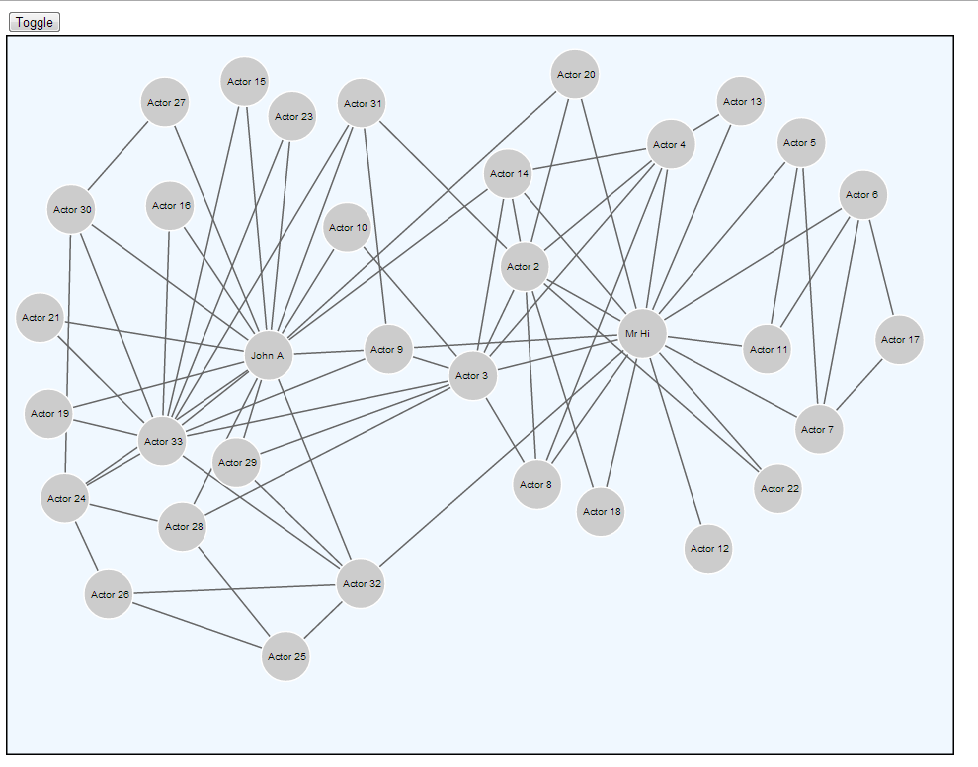
\includegraphics[width=1.00\textwidth]{karate-before.png}
	\caption{Zachary's Karate Club (Before)}
	\label{fig:karate-before}
\end{figure}


\begin{figure}[htbp]
	\centering
		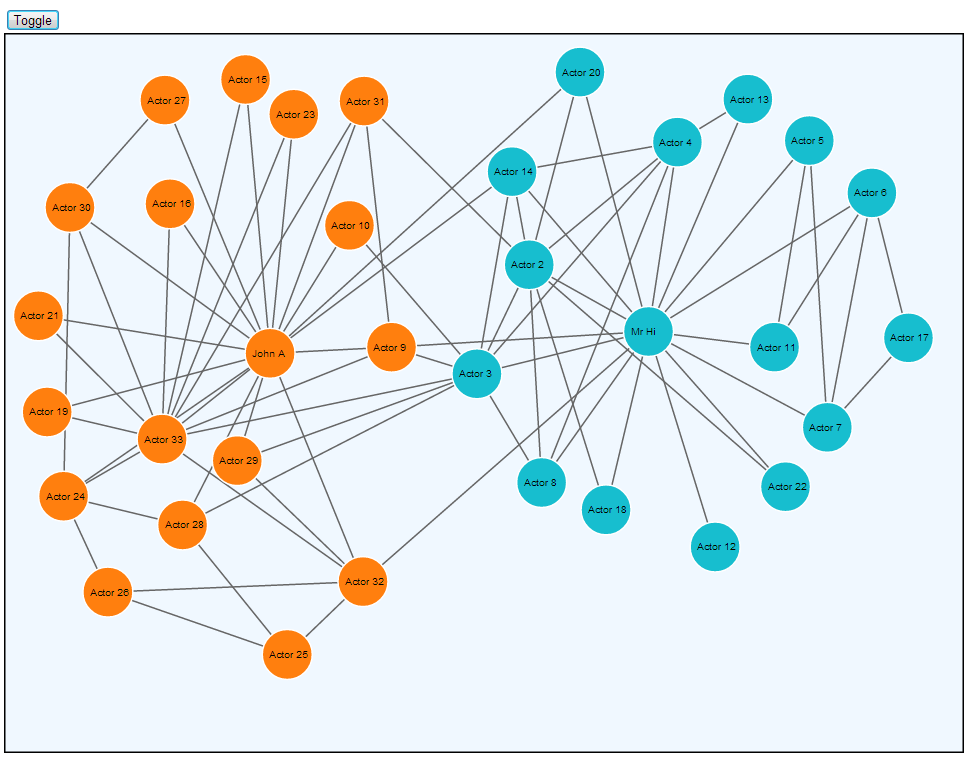
\includegraphics[width=1.00\textwidth]{karate-after.png}
	\caption{Zachary's Karate Club (After)}
	\label{fig:karate-after}
\end{figure}


%%%%%%%%%%Chapter Exercises
\section{Question 2 Extra Credit}
\subsection{Problem}Use D3 to create a who-follows-whom graph of your Twitter account.  Use my twitter account (``@phonedude\_mln'') if you do not have an interesting number of followers.
\subsection{Response}Did not attempt.


\end{savenotes}

% produce the bibliography for the citations in your paper.
\bibliographystyle{abbrv}
\bibliography{cmccoy}

\appendix
\addcontentsline{toc}{chapter}{Appendices}

%%Appendix A
\chapter{Python Source Code} \label{chap:Python}
\input{convertGraph.py}
\chapter{D3 Source Code} \label{chap:D3}
\input{index.html}


\end{document} 
%%%%%%%%%%Ed of report
